\chapter{Entwurf und Implementierung}
\label{cha:implementierung}

\todo{Kapitel-Einleitung}

\section{Modularer Architektur-Vorschlag}

%Komponenten des Brokers.
%
%
%In der CMP: Polling oder Notification?
%
%Was löst eine Aktion aus?
%- Monitoring der Services
%- Änderung der Umgebung
%- User-Aktion
%- Ergebnis einer anderen Policy

\begin{figure}
	\centering	
%	\def\svgwidth{0.95\textwidth}
%	{\tiny
%	\includesvg{images/broker-cycle}}
	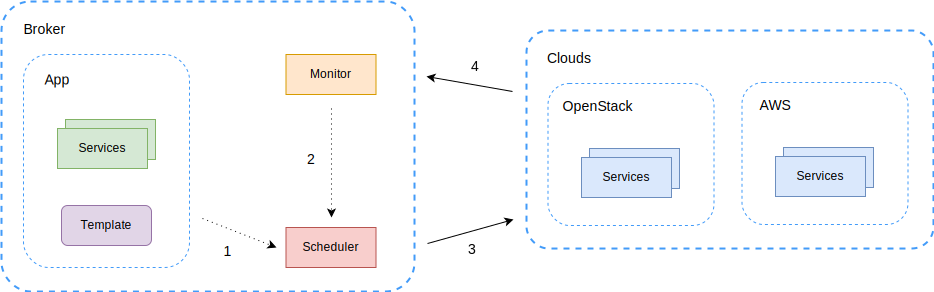
\includegraphics[width=\linewidth]{images/broker-cycle}
	\caption{Arbeitsweise des Multi-Cloud-Brokers als Zyklus: (1) Sammeln der Meta-Informationen aller Cloud-Provider, (2) Sammeln der Laufzeitinformationen der Anwendungen, (3) Sammeln der SLAs, (4) Nutzeränderungen: Neue Anwendungen oder Anpassung von SLAs, (5) Optimierungsplanung, (6) Planausführung auf den Cloud-Infrastrukturen}
	\label{fig:cycle}
\end{figure}

%Zyklus\autoref{fig:cycle}:

%\begin{description}
%	\item[Nummerierte Aufzählung]~\par
\begin{enumerate}
	
	\item Sammeln der Meta-Informationen alle Cloud-Provider
	\begin{enumerate}
		\item Kapazität (CPU, RAM, HDD, Network)
		\item Features (Verschlüsselung, CUDA, …)
		\item Geo-Lokation 
		\item Preis
	\end{enumerate}
	
	\item Sammeln der Laufzeitinformationen der PaaS/Anwendungen
	\begin{enumerate}
		\item Auslastung
		\item Fehler
		\item Ausfälle
	\end{enumerate}
	
	\item Sammeln der SLAs
	\begin{enumerate}
		\item Policy-Definitionen
		\item Policy-Konfiguration
		\item Placement-Algorithmen
	\end{enumerate}
	
	\item Neue Anwendung/Änderung eines SLA
	
	\item Optimierung
	\begin{enumerate}
		\item Feste Vorgaben (Geo, Backup)
		\item Weiche (Preis, Latenz, Verfügbarkeit)
	\end{enumerate}
	
	
	\item Ausführung
	\begin{enumerate}
		\item Netzwerkkonfiguration
		\item Allokation/De-Allokation von Ressourcen
		\item Deployment
		\item Migration
		\item Logging/Benachrichtigung
		\item Backup
	\end{enumerate}
	
\end{enumerate}

\section{Brokering}


%https://de.wikipedia.org/wiki/Constraintprogrammierung
%https://de.wikipedia.org/wiki/Scheduling

%entailing multiple constraint satisfaction (MCS)
%
%\todo{Schaubild, was wird wann gematcht}
%% Pseudocode des Algorithmus, wie in Meryn
%
%Kostenoptimierung
%
%Preisentwicklung? 
%
%Migration je nach Tageszeit? 
%
%Kosten der Datentransfers 
%
%Subscription On-Demand/Monthly/Yearly 
%
%Kompliziert durch undurchsichtige Staffelpreise
% https://www.rightscale.com/blog/cloud-cost-analysis/aws-vs-azure-vs-google-cloud-pricing-compute-instances

%https://www.rightscale.com/blog/cloud-cost-analysis/comparing-cloud-instance-pricing-aws-vs-azure-vs-google-vs-ibm

%
%Cost Calculators 
%
%http://go.appscale.com/cloud-cost-calculator-help 
%
%https://github.com/ifosch/accloudtant 
%
%https://awstcocalculator.com/# 
%
%Kosten: Rechenzeit und Bandbreite (außerhalb einer Cloud) also gegenläufiges Ziel zu Portabilität und Ausfallsicherheit, denn die geringsten Kosten fallen bei dem Betrieb in einer einzelnen Cloud eines Providers an.
%i) providers’ pricing models, (ii) application’s communication patterns and (iii) distribution of nodes over providers.
%https://www.google.de/url?sa=t&rct=j&q=&esrc=s&source=web&cd=1&ved=0ahUKEwju27vHs6DZAhUCWRQKHRv7BEcQFggrMAA&url=http%3A%2F%2Fwww.mikesmit.com%2Fwp-content%2Fpapercite-data%2Fpdf%2Fcloud2012.pdf&usg=AOvVaw3e6yhHYmhWBbIxtr7MqkuX


\input{content/4-3_hyrise-r.tex}

\input{content/4-4_openstack-testbed.tex}

\input{content/4-5_devstack-docker.tex}

\input{content/4-6_multi-cloud-bibliotheken.tex}


\section{Softwarearchitektur und Entwicklungsumgebung}


% Tatsächliche Broker Architektur
% Code-Eigenheiten
%as in Grozev 42: Federated CLoud Management: There is a central repository of images. this is replicated to the specific iaas/caas providers on demand.
%
%Alle weiteren Managementprozesse sind für Clients transparent.

\input{content/4-6_multi-provider-service-schema.tex}

\input{content/4-10_test.tex}

\section{Diskussion}

\todo{Mit Fazit zusammenlegen?}

%verschiedene OpenStack-Versionen haben unterschiedliche Schnittstellen. Auch dies kann über die Middleware abgefangen werden. RefStack testet API, Rally testet performance und führt tempest-Tests aus.


Aufwand einer Multi-Cloud-Strategie

Umsetzung der Policys

Potenzial

Vorteile durch Multi-Cloud-Bibliotheken

Aufwand für ein Multi-Cloud-Testbed

Redundanz fehlt: Auch die CMP muss in einer vertrauenswürdigen Umgebung repliziert werden und synchronisieren. Dem Hyrise-R-Dispatcher fehlt diese Funktion ebenso.